\documentclass[12pt]{article}

\usepackage{apacite}
\usepackage[longnamesfirst]{natbib}
\usepackage{geometry} %for setting up margins
\usepackage{url} %this package lets a url appear in the bibliography
\usepackage[english]{babel}
\usepackage[autostyle, english = american]{csquotes}
\MakeOuterQuote{"}  % the previous lines make it so that the quotation marks all appear the right way around 

%\usepackage{listings} %for inserting R scripts
%\usepackage{verbatimbox}

\usepackage{fancyvrb} %centre verbatim box

%for the figure stuff
\usepackage{subfig}
\usepackage{wrapfig}
%\usepackage{subfigure}
%\usepackage{subcaption}
\usepackage[justification=centering]{caption}
\usepackage[bottom]{footmisc}
% to set up the figures to be apa
%\captionsetup[figure]{labelsep=period,labelfont=it,justification=justified,singlelinecheck=false,font=doublespacing}
% add in font=doublespacing

\usepackage{fancyhdr} %Just used to make nice headers and footers 


\pagestyle{fancy}
\fancyhf{}
\fancyhead[LE,RO]{Penguins are cooler than you}
\fancyfoot[LE,LO]{Page \thepage}

\renewcommand{\headrulewidth}{2pt}
\renewcommand{\footrulewidth}{1pt}

\usepackage{graphicx}


\usepackage[normalem]{ulem} %this adds the \uline{} function which stops underlined titles from running off the page 
\usepackage{hyperref} % This package makes it so that your citations become hyperlinks to the web url provided or to the reference section... That's really cool [colorlinks=true,linkcolor=blue,citecolor=blue]

\geometry{a4paper, total={170mm,257mm}, left=20mm, top=20mm}
\usepackage{setspace}
\linespread{1.5} %says there's a problem but it seems to work for line spacing




\begin{document}

\begin{titlepage}
	\centering
	{\huge\bfseries Penguins are cool\par}
	\vspace{1cm}
	Warren \textsc{James}, \par
	Dr.~Josephine \textsc{Reuther}, \par
	Ellen \textsc{Angus}, \par
	Dr.~Amelia \textsc{Hunt},\par
	and\par
	Dr.~Alasdair \textsc{Clarke}
	\vfill
\end{titlepage}	


\newpage

%% ABSTRACT
\begin{center}
	\section*{Abstract}
\end{center}

\begingroup\singlespacing
\newpage
\tableofcontents
\newpage
\endgroup

%% Itroduction
\section*{Introduction}
\addcontentsline{toc}{section}{Introduction}

\section*{Methods}
\addcontentsline{toc}{section}{Methods}

\subsection*{Participants}
\addcontentsline{toc}{subsection}{Participants}
\paragraph{} Participants were recruited via word of mouth at the University of Aberdeen. \textit{Participant data is missing; I have details for 18 participants but there were 19 in the dataset. I'm assuming participant 25 was excluded as they only did 3 blocks instead of the full 4?} In total, 18 participants took part in the experiment (13 female) with an age range of 20-23 (mean of 20). 

\subsection*{Procedure}
\addcontentsline{toc}{subsection}{Procedure}
\paragraph{} The experiment took part over two sessions. The first session was to measure each participant's visual acuity in order to tailor the second session to each individual. The first session lasted approximately 30 minutes. In the second session, participants carried out the actual decision task, which lasted between 40 and 50 minutes. 

\paragraph{} Both sessions made use of and Eyelink 1000 (version 4.594) (\textit{get reference}) which recorded eye position at 1000 Hz. Participants were sat $\approx45cm$ from the screen, which was maintained throughout the experiment by use of an adjustable chin rest. \textit{Was this experiment on the OLED?}. The experiment was programmed and run in Matlab 7.9.0 (R2009b) with Psychtoolbox \textit{\textbf{get ref}} and EyelinkToolbox functions \textit{\textbf{get ref}}. Prior to starting each session, a 5-point calibration was carried out. Participants were recalibrated prior to starting a new block. Additionally, they were also recalibrated if they had failed to fixate appropriately 10 times since the last calibration, or if there were 5 errors in a row.

\subsubsection*{Session 1}
\paragraph{} In the first session, participants were presented with a fixation cross with two boxes placed either side \textit{\textbf{get fig}}. They were told that their task was to identify whether a small dot \textit{\textbf{get size of this dot}} had appeared in the top or the bottom half of one of the boxes (each $\approx1^{\circ}$). It did not matter which box it had appeared in, they were simply to report whether it was up or down by pressing the "up" or "down" arrow, respectively, on the keyboard. To commence each trial, participants had to press the space bar whilst fixating the central cross. After maintaining fixation for 700ms, the target dot would appear in one of the two boxes, at random, and was displayed for 700ms (\textit{\textbf{Need to double check all this}}). If participants broke fixation during any stage of this process, the screen would turn red for 700ms to indicate that they had broken fixation. 

\paragraph{} The boxes were presented at varying separations from the central fixation cross ($2.7^{\circ}$, $3.9^{\circ}$, $5.2^{\circ}$, $6.8^{\circ}$, $8.4^{\circ}$, $10.1^{\circ}$, $11.4^{\circ}$, $12.5^{\circ}$). There were 4 blocks in total, with each different separation being presenter 12 times in a pseudo-random order. This meant participants completed 4 blocks of 96 trials. Data from this session was then used to work out the point at which participants were 75\% accurate in detecting the target. This value was then used in the second session to tailor the experiment for each individual.

\subsubsection*{Session 2}  
\paragraph{} For the second session, participants were introduced to "\textit{Pugadoo}". They were told that there task was to help Pugado collect as many fish as possible. In order to do this, they would be choosing a box to fixate in order to detect whether the target dot was in the upper or lower half of one of the two side boxes (\textit{\textbf{Get fig}}). On each trial, participants would see Pugadoo and have to fixate the star on their stomach to start the trial. They would then press the space bar and three boxes would appear. Participants were told they could fixate any one of the three boxes but that the target would only ever appear in one of the two side boxes at random. These boxes were placed at various distances from the centrally presented box. These distances were defined in relation to the switch point that was calculated based on their performance in the first session. Seven were defined as the switch point in the following way; switch point $-3^{\circ}$, $-2^{\circ}$, $-1^{\circ}$, $0^{\circ}$, $+1^{\circ}$, $+2^{\circ}$, $+3^{\circ}$. A further two distances were added so as to be constants across all participants ($8^{\circ}$ and $18^{\circ}$). 

\paragraph{} For every trial that the participants correctly identified the position of the target dot, the background would turn green and the bar in the top left corner would fill by one tick. After having filled the bar to the top, Pugadoo would be rewarded with a fish and the bar would return to being halfway filled. If the participant was incorrect, the background would turn red and the bar would be emptied by one tick on the bar. If the bar was fully depleted, a fish would be taken away from the total. This allowed participants to monitor their performance while completing the task. 

\paragraph{}

\section*{Results}
\addcontentsline{toc}{section}{Methods}
\begin{figure}[ht!]
	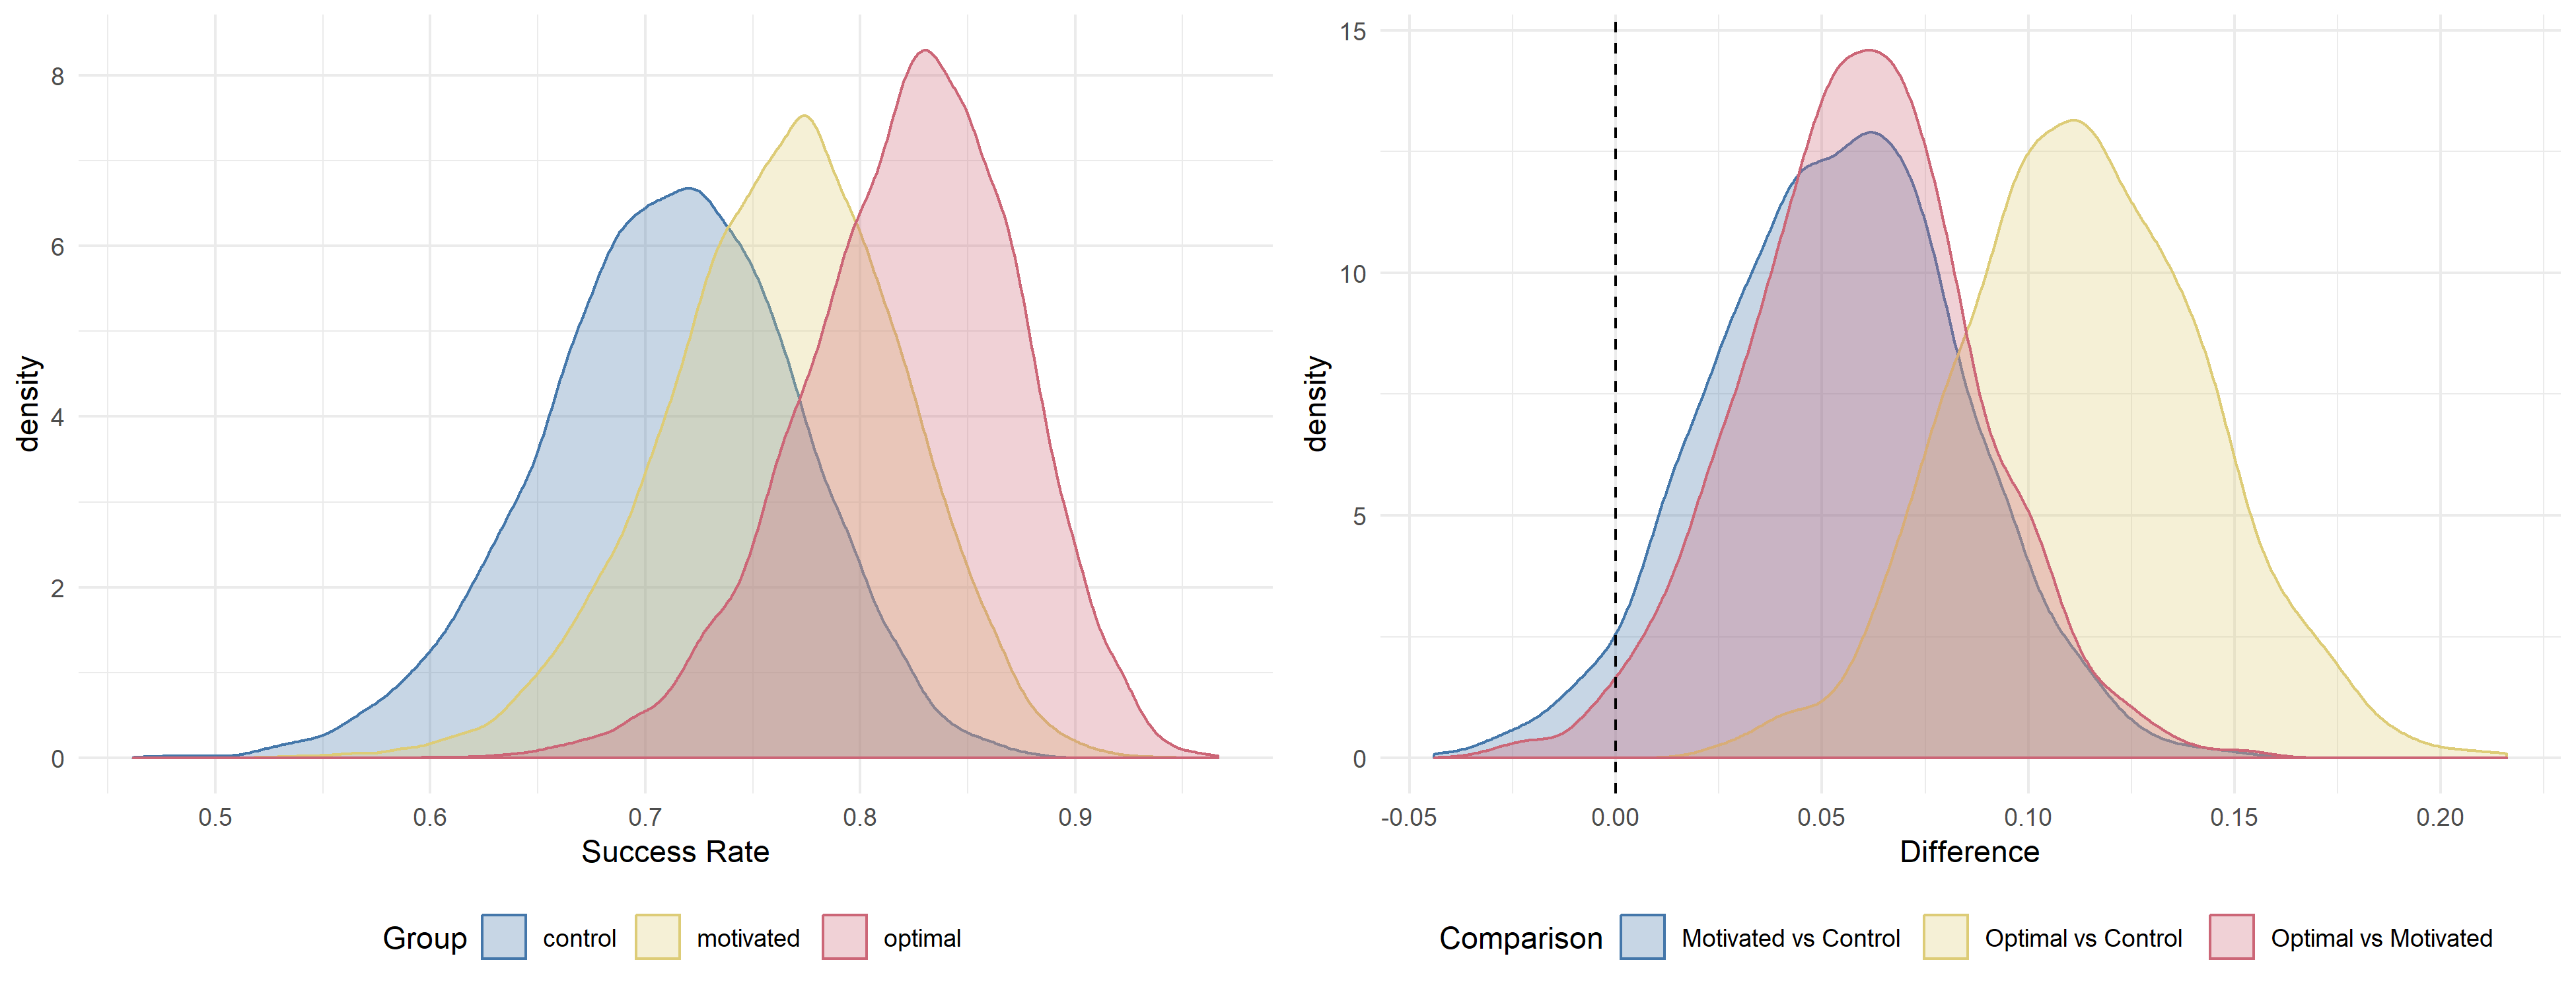
\includegraphics[scale=0.5]{../Figures/Model_output_raw_acc.png}
	\centering
	\captionsetup{justification=centering}
	\caption{Model output for raw success rate}
	\label{fig:Model_raw_acc}
\end{figure}

\begin{figure}[ht!]
	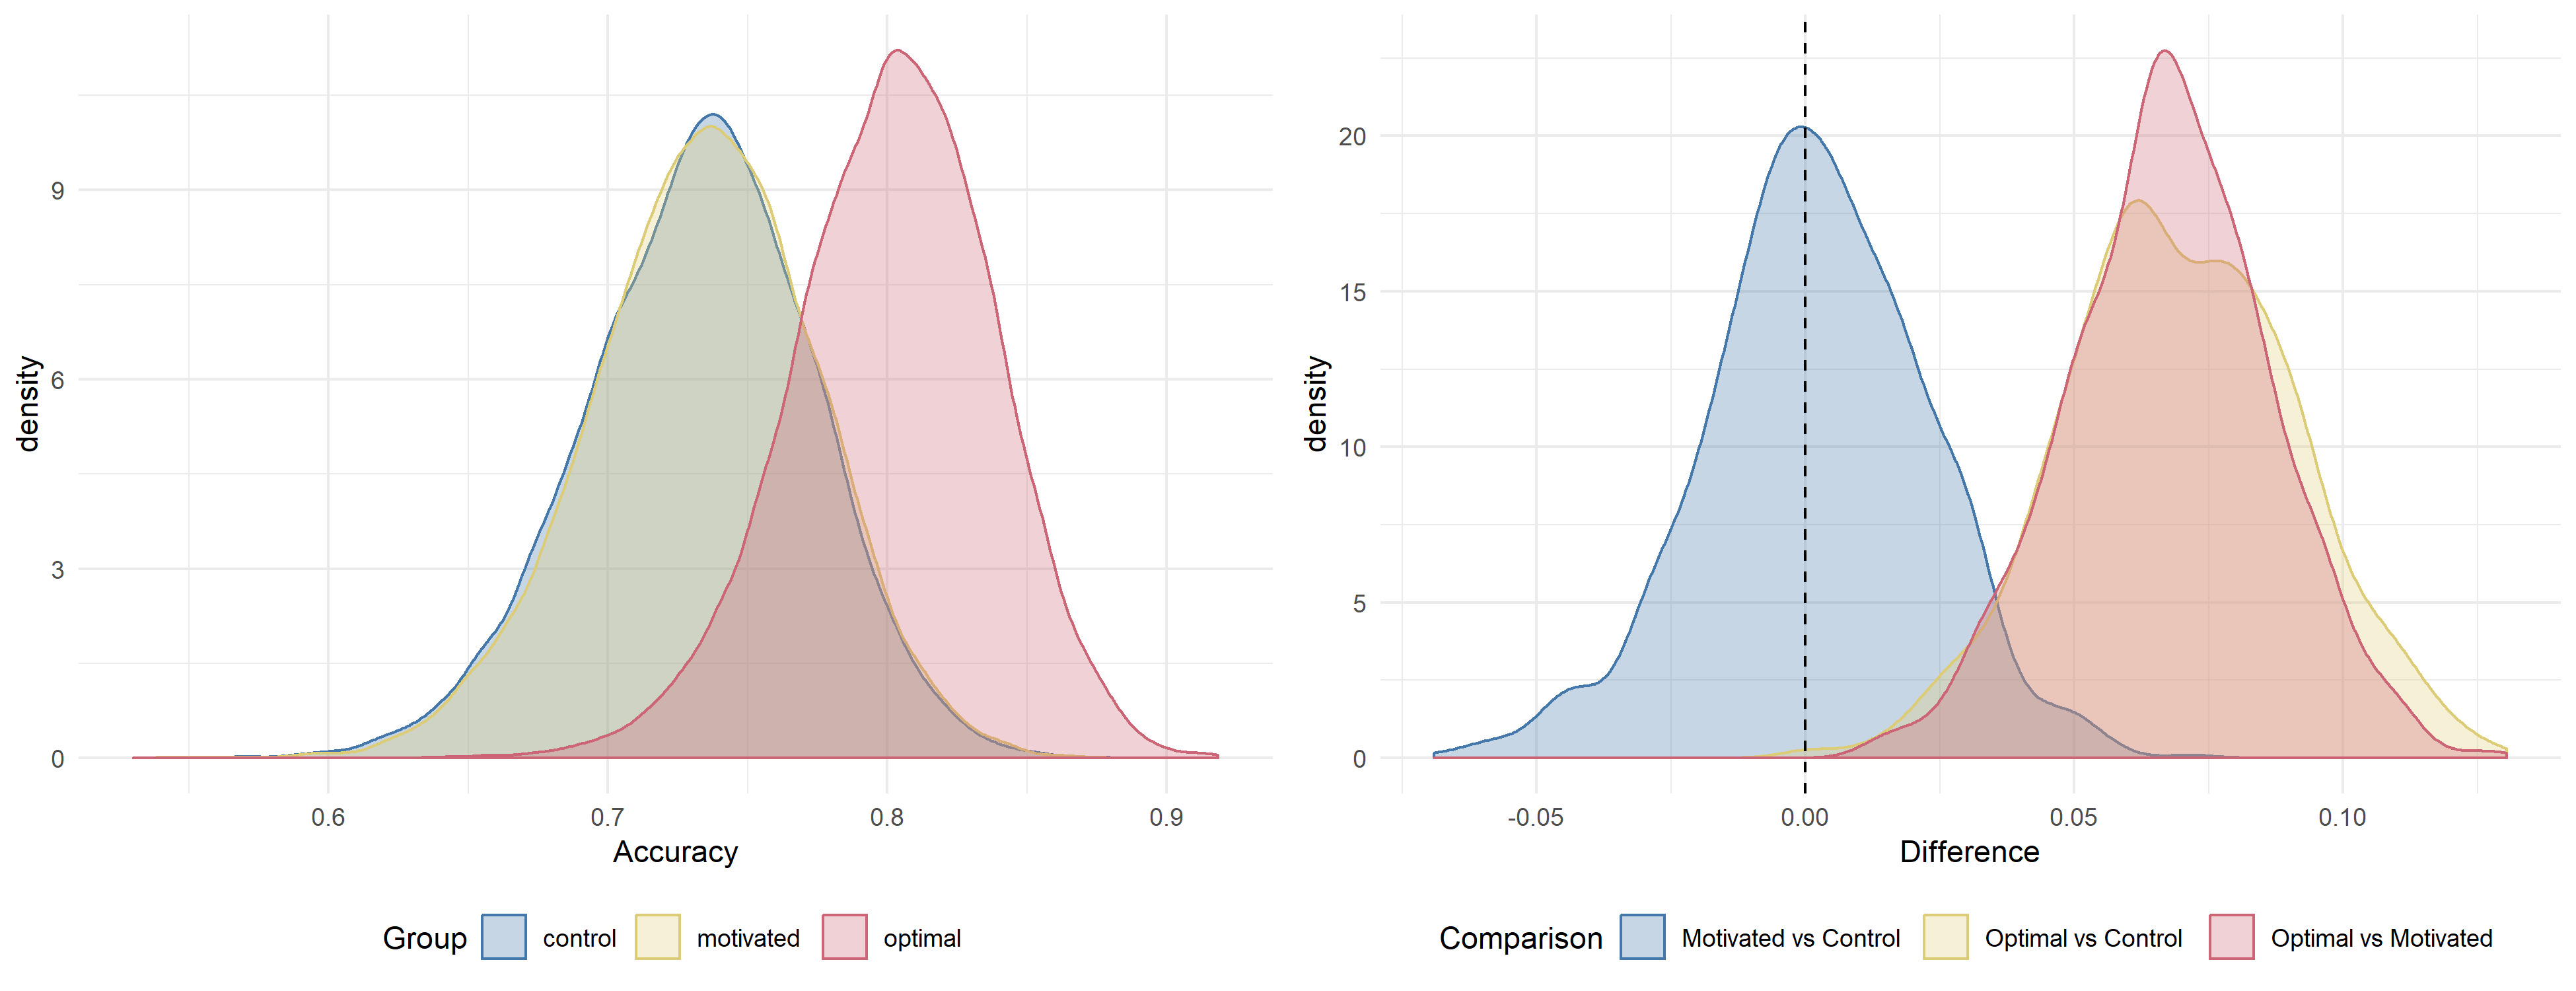
\includegraphics[scale=0.5]{../Figures/Model_output_exp_acc.png}
	\centering
	\captionsetup{justification=centering}
	\caption{Model output for expected success rate}
	\label{fig:Model_exp_acc}
\end{figure}
\section*{Discussion}
\addcontentsline{toc}{section}{Discussion}

\section*{Conclusion}
\addcontentsline{toc}{section}{Conclusion}

\end{document}